\documentclass{article}

\usepackage{graphicx}
\usepackage{tikz}
\usepackage{tikzsymbols}
\usetikzlibrary{calc,patterns,shapes.geometric}
\pagestyle{empty}
\usepackage[margin=0pt]{geometry}
\geometry{papersize={14in,12in}}

\def\centerarc[#1](#2)(#3:#4:#5){\draw[#1] ($(#2)+({#5*cos(#3)},{#5*sin(#3)})$) arc (#3:#4:#5);}

\begin{document}
	\begin{figure}
		\centering
		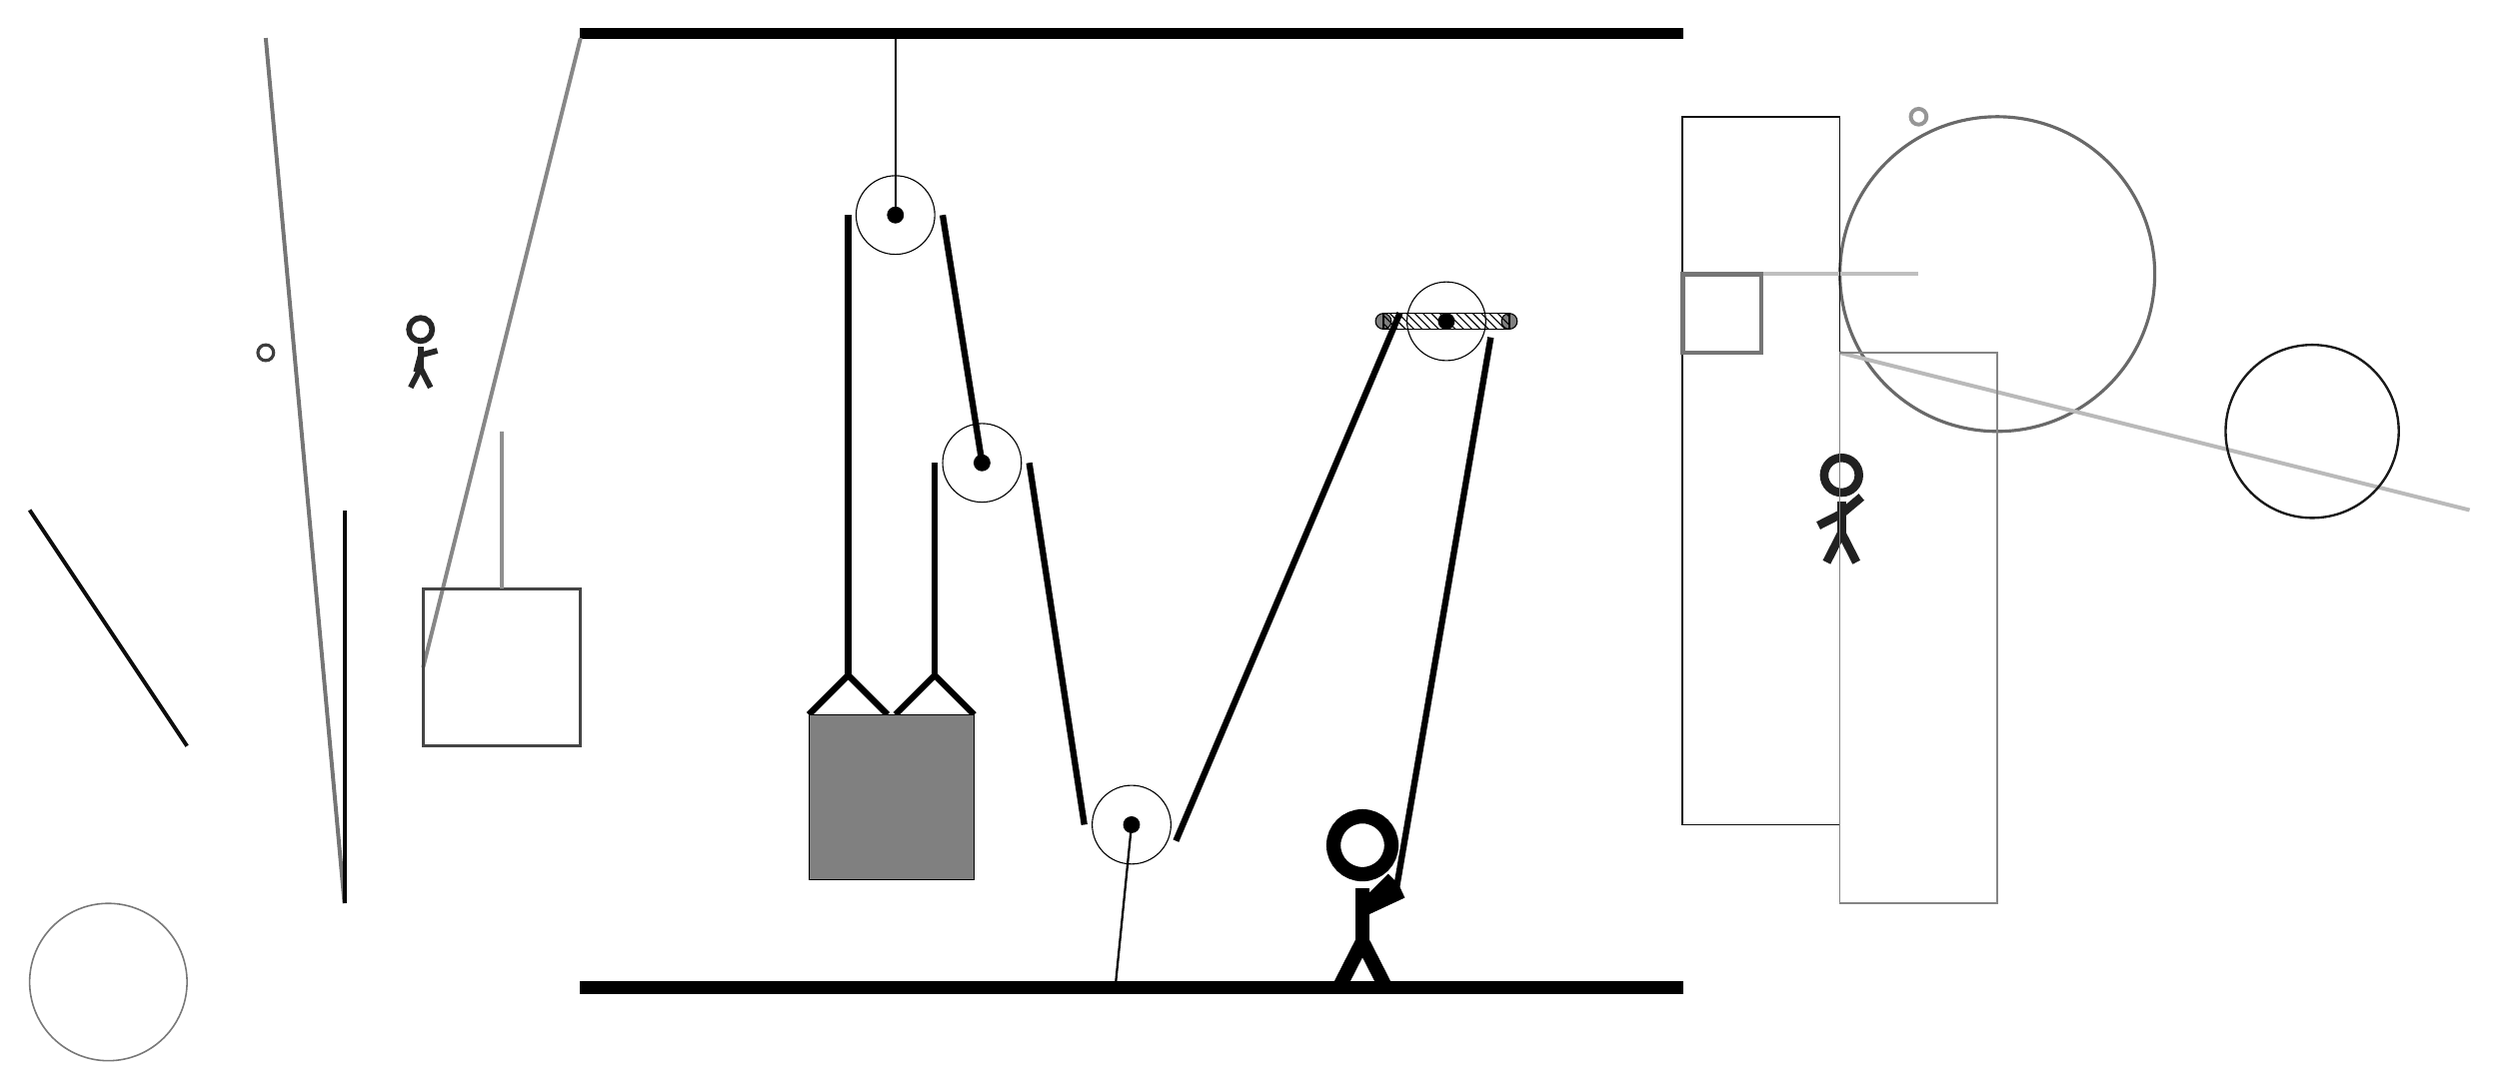
\begin{tikzpicture}
			%%%%% START %%%%%
			
			\draw[fill=black] (-2, 9) rectangle (12, 9.125);
			
			\draw (2, 6.75) circle (0.5);
			\draw[fill=black] (2, 6.75) circle (0.1);
			\draw[thick] (2, 6.75) -- (2, 9);
			
			\draw[line width=0.5mm, color=black!47](-2, 9) -- (-4, 1);
			
			\node[line width=0.5mm, color=black!87] at (14, 3) {\Strichmaxerl[6][27][40]};
			\draw [line width=0.4mm, color=black!59](16, 6) circle (2.0);
			\draw[line width=0.5mm, color=black!27](14, 5) -- (22, 3);
			\draw[line width=0.5mm, color=black!54](-6, 9) -- (-5, -2);
			\draw [line width=0.2mm, color=black!53](-8, -3) circle (1.0);
			\draw[line width=0.5mm, color=black!95](-7, 0) -- (-9, 3);
			\draw[line width=0.4mm, color=black!73] (-2, 2) rectangle (-4, 0);
			\node[line width=0.6mm, color=black!85] at (-4, 5) {\Strichmaxerl[4][75][15]};
			
			\draw[line width=0.5mm, color=black!25](13, 6) -- (15, 6);
			\draw[line width=0.2mm, color=black!93] (12, 8) rectangle (14, -1);
			\draw[line width=0.5mm, color=black!97](-5, -2) -- (-5, 3);
			\draw [line width=0.5mm, color=black!41](15, 8) circle (0.1);
			\draw [line width=0.4mm, color=black!76](-6, 5) circle (0.1);
			\draw[line width=0.6mm, color=black!54] (13, 5) rectangle (12, 6);
			\draw[line width=0.2mm, color=black!48] (14, -2) rectangle (16, 5);
			\draw[line width=0.5mm, color=black!44] (-3, 4) rectangle (-3, 2);
			\draw [line width=0.3mm, color=black!90](20, 4) circle (1.1);
			
			\draw (3.1, 3.6) circle (0.5);
			\draw[fill=black] (3.1, 3.6) circle (0.1);
			
			\draw (5, -1) circle (0.5);
			\draw[fill=black] (5, -1) circle (0.1);
			\draw[thick] (5, -1) -- (4.8, -3);
			
			\draw (9, 5.4) circle (0.5);
			\draw[fill=black] (9, 5.4) circle (0.1);
			\draw[fill=black!50] (8.2, 5.4) circle (0.1);
			\draw[fill=black!50] (9.8, 5.4) circle (0.1);
			\draw[pattern=north west lines, pattern color=black] (8.2, 5.5) rectangle (9.8, 5.3);
			
			\draw[line width = 0.8mm]  (0.9, 0.4) -- (1.4, 0.9) -- (1.9, 0.4);
			\draw[line width = 0.8mm]  (2.0, 0.4) -- (2.5, 0.9) -- (3.0, 0.4);
			\draw[fill=black!50] (0.9, 0.4) rectangle (3.0, -1.7);
			
			\draw[line width = 0.8mm] (1.4, 6.75) -- (1.4, 0.9);
			\centerarc[line width = 0.8mm](2, 6.75)(0:180:0.6);
			\draw[line width = 0.8mm] (2.6, 6.75) -- (3.1, 3.6);
			\draw[line width = 0.8mm] (2.5, 3.6) -- (2.5, 0.9);
			\centerarc[line width = 0.8mm](3.1, 3.6)(0:180:0.6);
			\draw[line width = 0.8mm] (3.7, 3.6) -- (4.4, -1);
			\centerarc[line width = 0.8mm](5, -1)(180:340:0.6);
			\draw[line width=0.8mm](5.5638, -1.2052) -- (8.4091, 5.5042);
			\centerarc[line width = 0.8mm](9, 5.4)(-20:170:0.6);
			\draw[line width=0.8mm](9.5638, 5.1948) --  (8.35, -1.9);
			
			\node at (8, -2) {\Strichmaxerl[10][225][25]};
			
			\draw[fill=black] (-2, -3) rectangle (12, -3.15);
			
			%%%%% END %%%%%
		\end{tikzpicture}
	\end{figure}	
\end{document}